\begin{Exercise}[label=heate, origin = {US IPhO Auswahlwettbewerb, Halbfinale 2013}, title = Wärmetauscher,difficulty = 4]
Die durch Wärmeleitung übertragene Wärmeleistung zwischen zwei parallelen Wänden kann näherungsweise durch die Gleichung 
\begin{equation}\label{he:fg}
	P = \lambda A \frac{T_a-T_b}{d}
\end{equation}
beschrieben werden. Dabei ist $A$ die Fläche, durch die Wärme strömt, $d$ der Abstand zwischen den beiden Wänden und $\lambda$ eine Konstante, die vom Material zwischen den beiden Wänden abhängt (die sog. Wärmeleitfähigkeit). $T_a$ ist die Temperatur der wärmeren Wandoberfläche und $T_b$ die der kälteren Wandoberfläche.\\
Ein Wärmetauscher ist ein Gerät, dass Wärme von einer warmen Flüssigkeit zu einer kälteren Flüssigkeit überträgt (Abb. \ref{fig:heate}).
Dabei fließt warme Flüssigkeit (rot) mit einer Geschwindigkeit $v$ von rechts nach links, und kalte Flüssigkeit (blau) mit einer Geschwindigkeit von $v$ von links nach rechts. Die Dichte der Flüssigkeiten ist $\rho$ und die Wärmekapazität $c$. Beide befinden sich in Röhren der Höhe $h$ ($h$ ist sehr klein).  Die beiden Flüßigkeiten sind durch eine Metallwand (grau) der Dicke $d$ mit der Wärmeleitfähigkeit $\lambda$ getrennt. \\
Die Temperaturdifferenz zwischen der einfließenden warmen Flüssigkeit und der einfließenden kalten Flüssigkeit beträgt $\Delta T_e$. \\
Bestimme die Temperaturdifferenz zwischen der abgekühlten, ausfließenden warmen Flüssigkeit und der aufgewärmten, ausfließenden kalten Flüßigkeit, $\Delta T_a$. Nimm dafür an, dass die Temperaturdifferenz $\Delta T$ zwischen warmer und kalter Flüssigkeit entlang der Wand konstant bleibt.

\end{Exercise}
\begin{figure}[h]
	\centering
	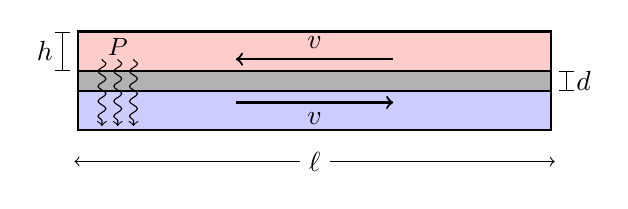
\begin{tikzpicture}

\filldraw[thick, draw = black, fill = red!20!white] (-3,-0.25)rectangle (3,.25);
\filldraw[thick, draw = black, fill= black!30!white] (-3,-0.5)rectangle (3,-.25);
\filldraw[thick,draw= black, fill=blue!20!white] (-3,-1)rectangle(3,-.5);

\draw[|-|] (3.2,-.25)--(3.2,-.5) node [midway, right] {$d$};

\draw[->,thick] (-1,-.65) -- (1,-.65) node[midway, below] {$v$};
\draw[<-,thick] (-1,-.1)--(1,-.1) node[midway, above]{$v$};
\draw[->,decorate,decoration={snake, amplitude = 0.5mm, segment length = 1.9mm}] (-2.5,-0.1) -- (-2.5,-.95);
\draw[->,decorate,decoration={snake, amplitude = 0.5mm, segment length = 1.9mm}] (-2.7,-0.1) -- (-2.7,-.95);
\draw[->,decorate,decoration={snake, amplitude = 0.5mm, segment length = 1.9mm}] (-2.3,-0.1) -- (-2.3,-.95);
\node at (-2.5,0.05) {\small $P$};
\draw[|-|] (-3.2,.25)--(-3.2,-.25) node[midway, left]{$h$};
\draw[<->] (-3.05,-1.4) -- (3.05,-1.4) node[midway, fill = white] {$\ell$};
\end{tikzpicture}
	\caption{Ein Wärmetauscher}
	\label{fig:heate}
\end{figure}
\begin{Answer}[ref= heate]
	Die warme (rote) Flüssigkeit strömt mit einer Temperatur $T_{r,e}$ in den Wärmetauscher und verlässt ihn mit einer Temperatur $T_{r,a}$. Diese Temperaturänderung  $\Delta T_r$ kommt durch den Wärmeaustausch mit der Leistung $P$ aus \eqref{he:fg}. 
	Die Leistung ist definiert als die Wärmezufuhr pro gegebener Zeiteinheit, also $P = \frac{Q}{t}$. Die Zeit $t$, in der hier die rote Flüssigkeit Wärme abgibt, ist genau die Zeit, die gebraucht wird, um die Röhre des Wärmetauschers zu durchlaufen, also $ t = \frac{\ell}{v}$. In dieser Zeit fließt eine Masse von $m = \rho V = \rho A h$ durch den Wärmetauscher, wobei $A$ genau die Fläche ist, über die die Wärmeübertragung stattfindet. Die Temperaturänderung $\Delta T_r$ kann also über die abgegebene Leistung berechnet werden zu
	\begin{equation}\label{he:tloss}
		P = -\frac{Q}{t} = \frac{m c \Delta T_r}{t} \Rightarrow \Delta T_r =- \frac{Pt}{mc} \overset{\eqref{he:fg}}{=} \underbrace{\frac{\lambda A \Delta T }{d}}_{=P}\cdot \underbrace{\frac{\ell}{v}}_{= t}\cdot \underbrace{\frac{1}{\rho c A h}}_{=\frac{1}{mc}} = -\frac{\lambda \Delta T\ell}{dv\rho c h}.
	\end{equation}
	Da wir die Temperatur der ausfließenden roten Flüssigkeit $T_{r,a}$ auch durch die der einfließenden kalten Flüssigkeit $T_{k,e}$ und die (konstante) Temperaturdifferenz zwischen den beiden Wänden $\Delta T$ ausdrücken können, ist
	\begin{equation}\label{he:dtr}
		\Delta T_{r} = T_{r,a} - T_{r,e} = T_{k,e}+\Delta T - T_{r,e} = \Delta T - \Delta T_e,
	\end{equation}
	wobei $\Delta T_e$ die Temperaturdifferenz der einfließenden Flüssigkeiten ist. 
	Wir können \eqref{he:tloss} und \eqref{he:dtr} gleichsetzten, und so die Temperaturdifferenz zwischen den Wänden bestimmen
	\begin{equation}\label{he:tdiffwall}
	-\frac{\lambda \Delta T\ell}{dv\rho c h} = \Delta T - \Delta T_e \Rightarrow \Delta T \left(1+\frac{\lambda \ell}{dv\rho c h}\right) = \Delta T_e\Rightarrow \Delta T = \Delta T_e \left(1+\frac{\lambda \ell}{dv\rho c h}\right)^{-1}.
	\end{equation}
	Durch $\Delta T$ können wir jetzt die gesuchte Temperaturdifferenz zwischen den ausfließenden Flüssigkeiten $\Delta T_a$ finden. Es ist 
	\begin{equation}
	\boxed{
		\Delta T_a = T_{r,a} - T_{k,a} = T_{k,e} + \Delta T - \left(T_{r,e}-\Delta T\right) = 2\Delta T - \Delta T_{e} =\Delta T_e\left( \frac{2}{1+\frac{\lambda \ell}{dv\rho c h}}-1\right).}
	\end{equation}
\end{Answer}